%!TEX root = ../thesis.tex
\section{SOFTWARE REQUIREMENTS SPECIFICATION}

The software development process starts with writing a software requirements specification (SRS)
so that
it serve as an agreement between client and contractor about the set of the
features which need to be implemented. Another important purpose of this document
is to create understanding of the features with higher and lower priority, thus developer
would know what should be implemented in the first version of the product and what could
be added later.

In this section the simplified version of the SRS will be presented which includes description
of the user interface, operating environment, and set of system features with detailed
explanation.

\subsection{Graphical User Interface}

The interface design was provided by Mathrioshka LLC, which includes set of different states
of the application with small description provided. The interface should have been implemented
to work in browser with use of HTML5 standard. The whole program should be implemented
as single page application, which means that all changes in the state of the application
happen without page reload. The interface have to be responsive and support screen sizes
starting from $800 \times 600$ pixels.

The manipulation of the data within the application is performed utilizing main control elements.
Most important elements are listed below:

\begin{enumerate}
  \item Mode selector is needed for switching from general overview to location-wise analysis and
  located in the left bottom corner of the screen.

  \begin{figure}[ht]
    \centering
    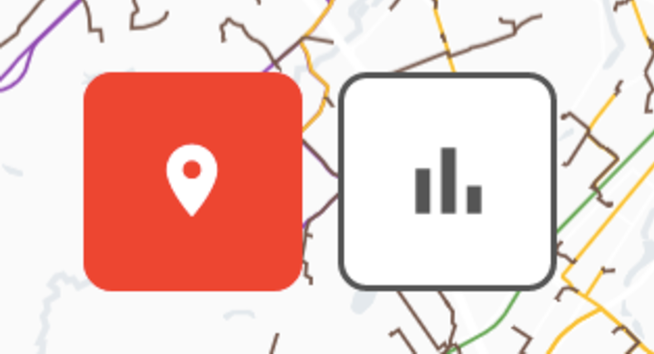
\includegraphics[width=0.33\textwidth]{mode-selector.pdf}
    \caption{Mode selector.}
    \label{pic:mode_selector}
  \end{figure}

  \item Overview mode selector switches different types of overview analysis tools. For some
  views it has embedded slider used for filtering. The component is positioned on the right
  side of the screen.

  \begin{figure}[ht]
    \centering
    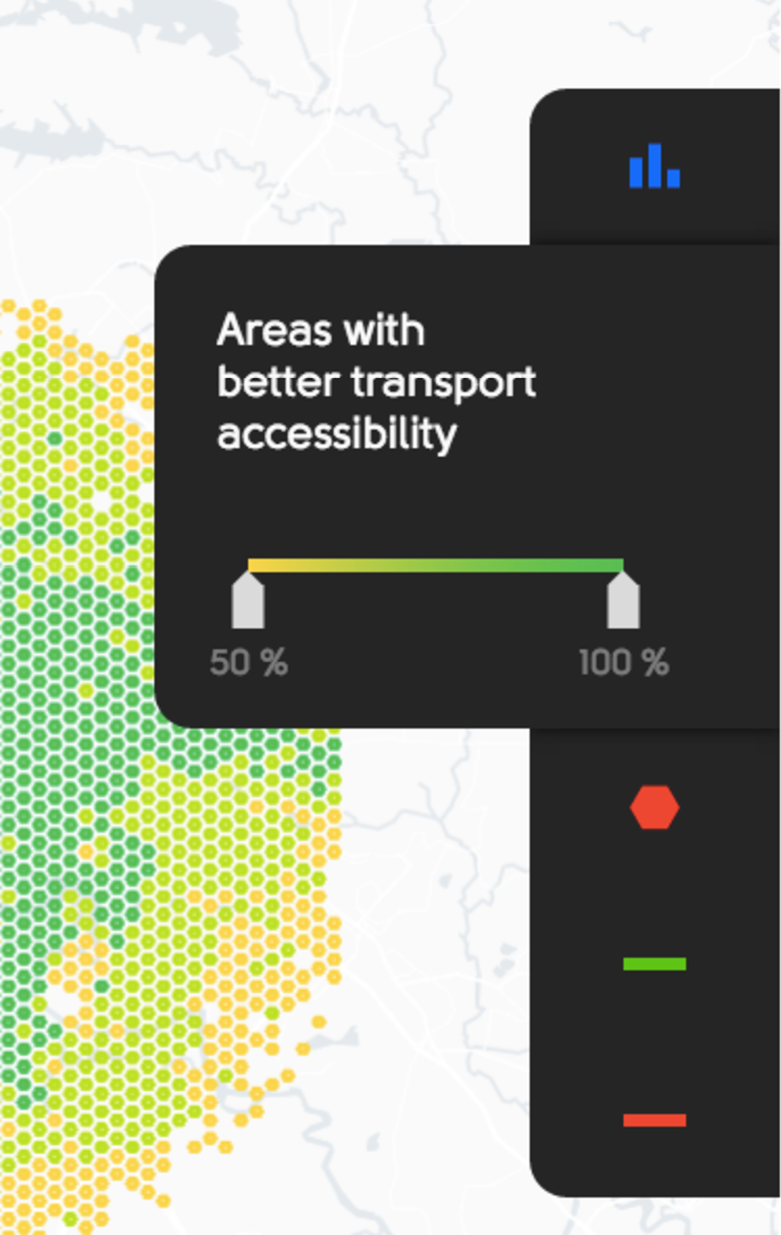
\includegraphics[width=0.25\textwidth]{overview-mode.pdf}
    \caption{Overview mode selector.}
    \label{pic:overview_selector}
  \end{figure}

  \item Transport filter is a set of checkboxes where every checkbox represent certain
  type of transport. This component is placed on top of the screen.

  \begin{figure}[ht]
    \centering
    
\includegraphics[width=0.8\textwidth]{transport-filter.pdf}
    \caption{Transport filter.}
    \label{pic:transport_filter}
  \end{figure}

  \item Current location indicator shows what point is selected on the map at this moment and
  also allows to clear current selection. The component is located on the right side of the window.

  \begin{figure}[ht]
    \centering
    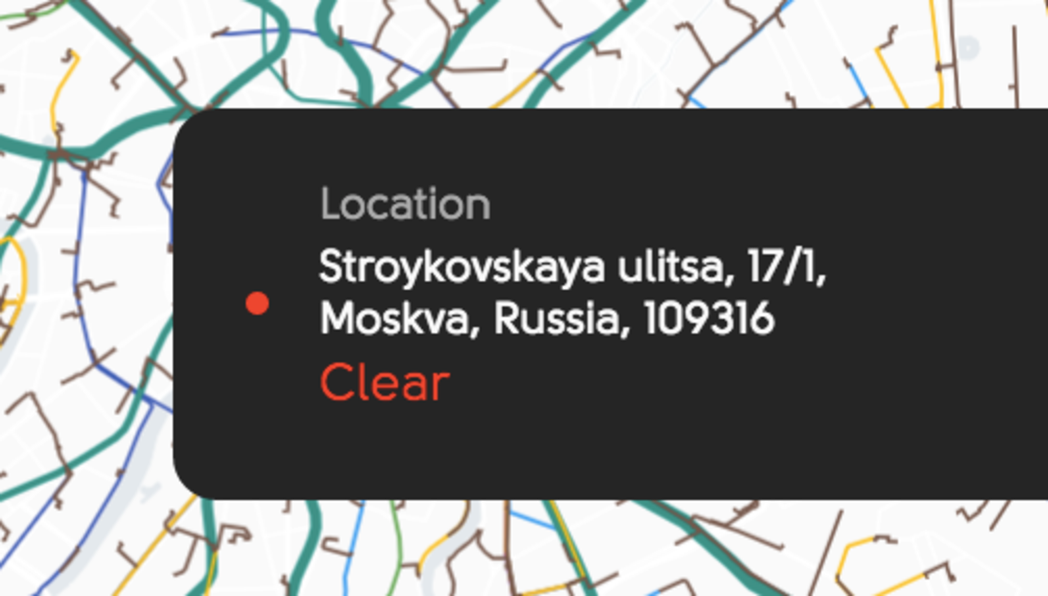
\includegraphics[width=0.3\textwidth]{location-selector.pdf}
    \caption{Current location indicator.}
    \label{pic:transport_filter}
  \end{figure}

  \item Map is the most important element of the interface which is presented on every screen
  of the application the only thing that changes is the content of the map.
  This component can show points, areas, routes and also provides functionality for
  selecting particular locations for analysis.

  \begin{figure}[ht]
    \centering
    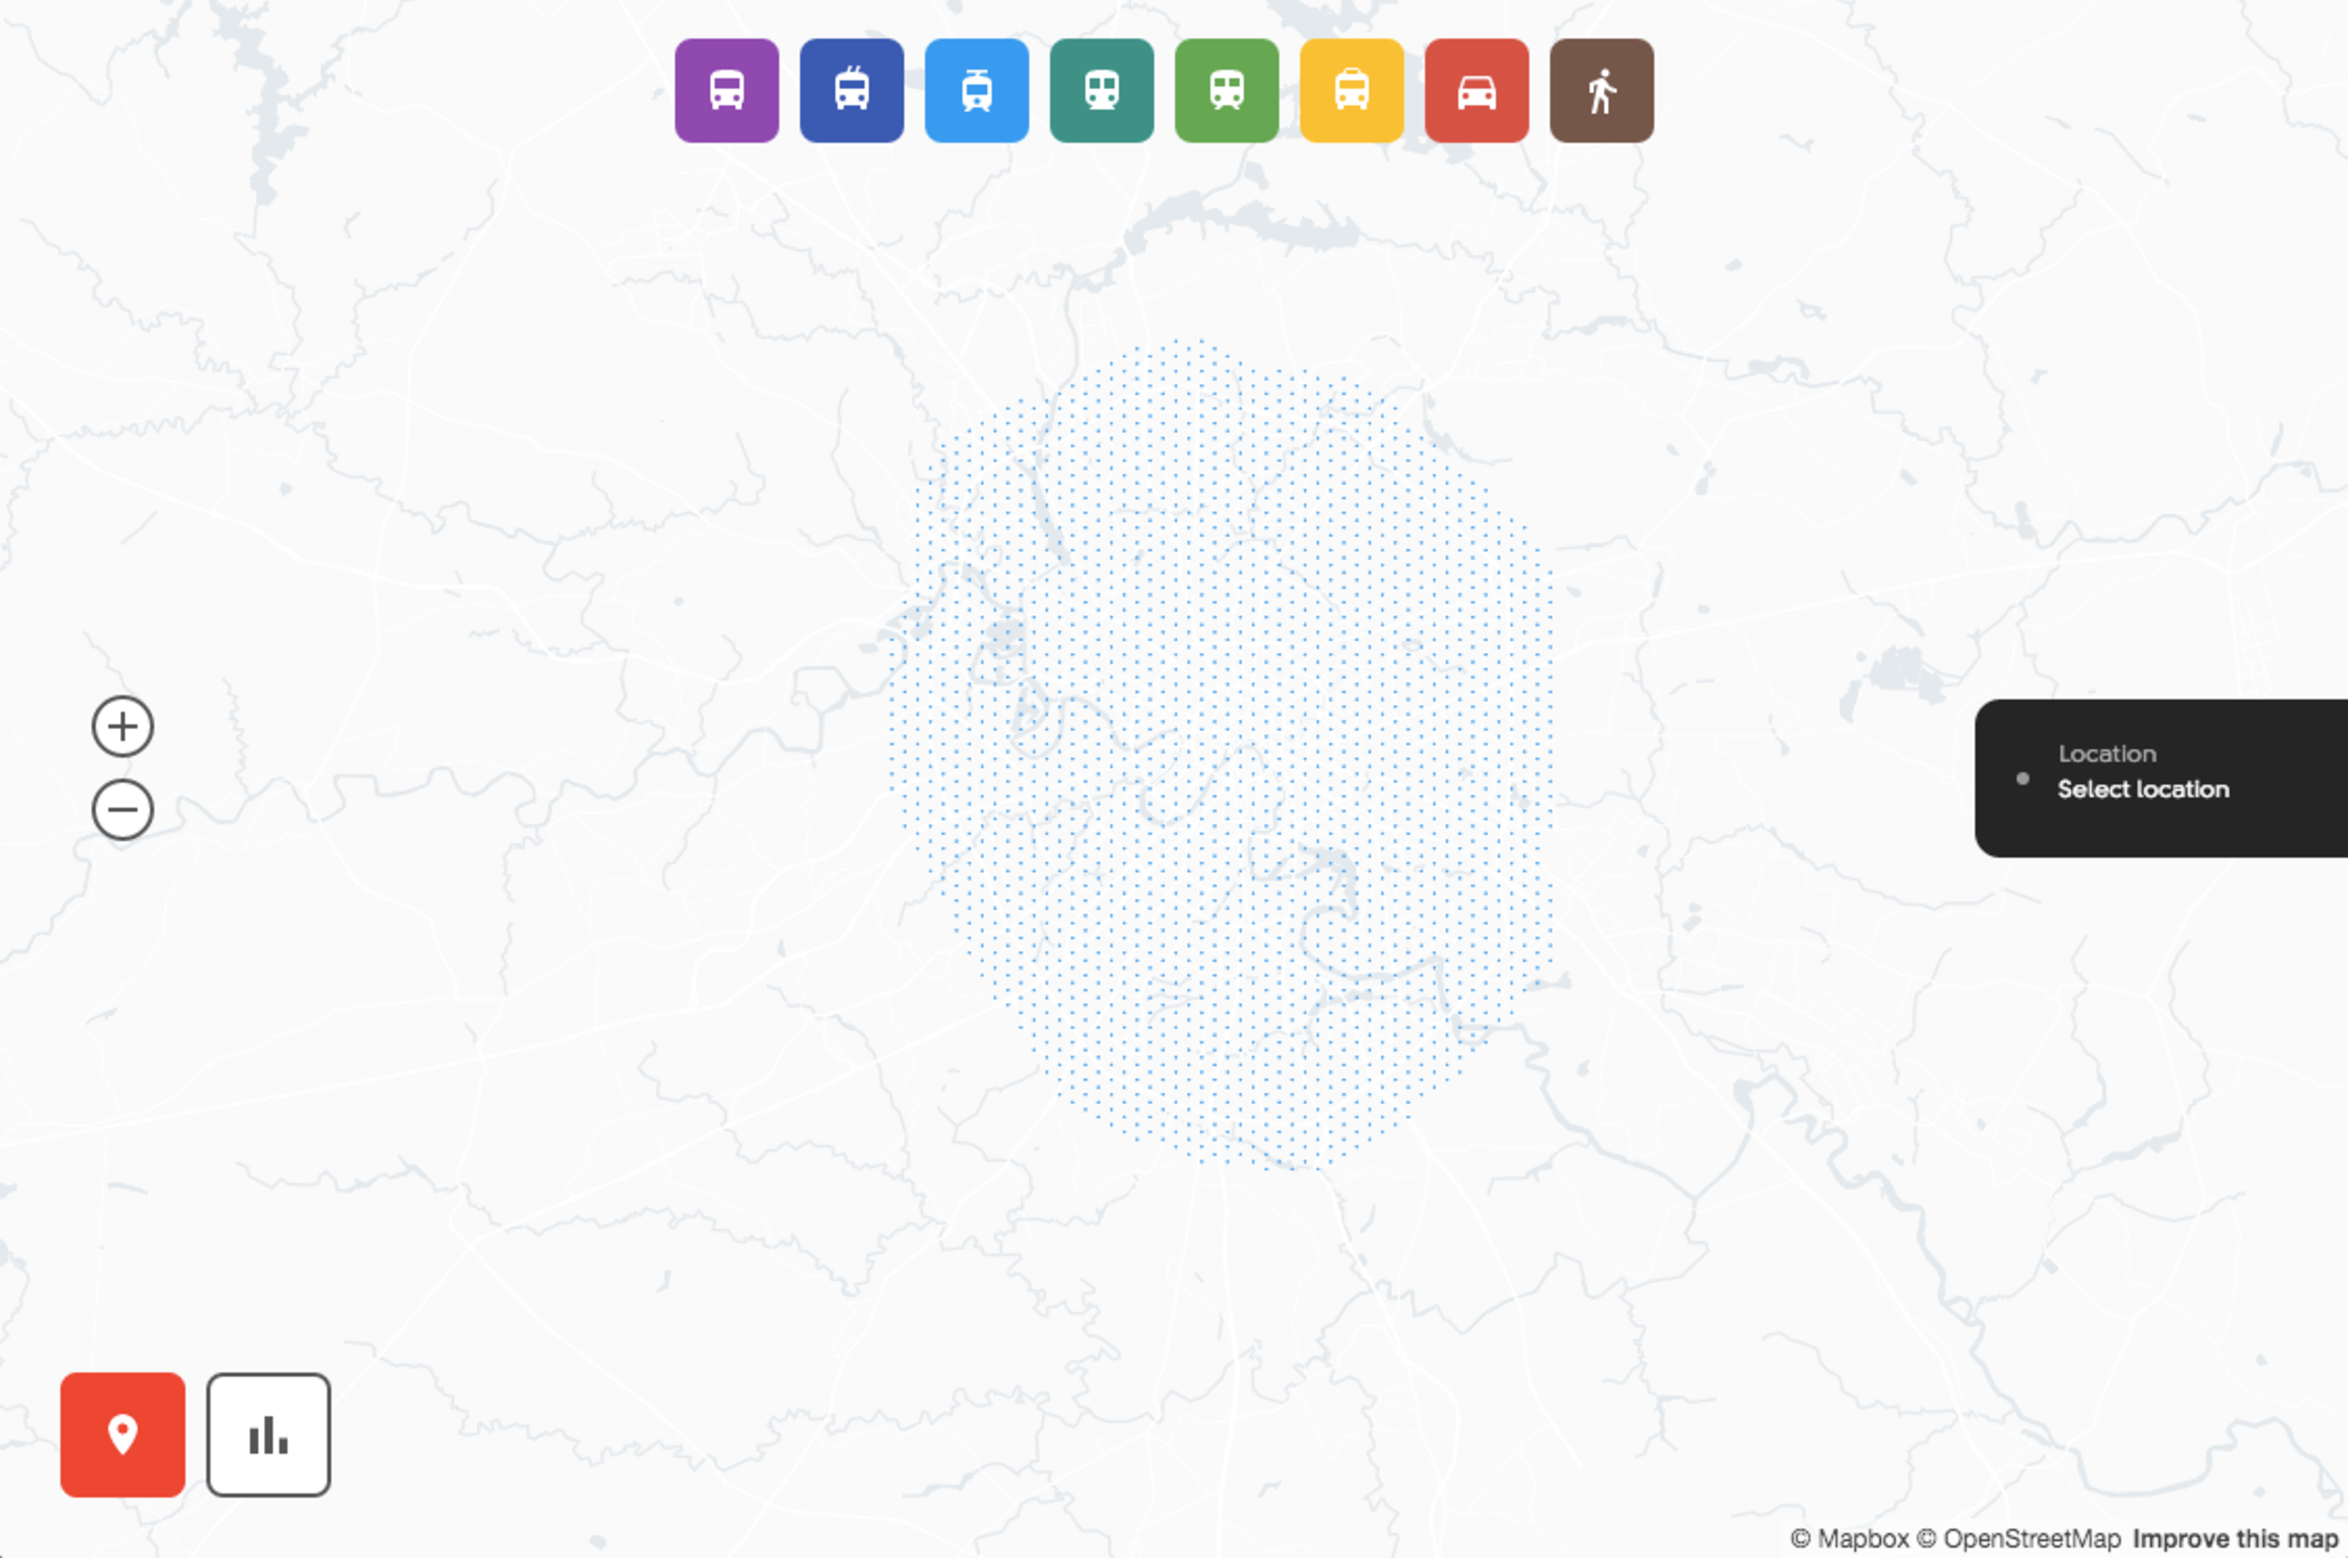
\includegraphics[width=0.80\textwidth]{map.pdf}
    \caption{Map.}
    \label{pic:map}
  \end{figure}

\end{enumerate}

\subsection{Operating Environment}

The software is developed on x86 based computer using Mac OS X 10.11 operating system. The
computer hardware is featured 8~GB 1600~MHz DDR3 RAM and 1.6 GHz Intel Core i5 processor.
The client should operate on any system which is able to install browsers like Google Chrome~49.0,
Safari, Firefox or Microsoft Edge. Hence it works well on Windows, Mac OS X and Linux. As for the
server, it was tested to work on Ubuntu~14.04 and 512~Mb~RAM. Running the server side on Windows
was not tested.

\subsection{System Features}

\begin{description}
  \item[Use case 1:] Hello there this is the first use case... bla bla bla...
\end{description}